\documentclass[border={7pt 0pt 7pt 0pt},varwidth]{standalone}
\usepackage{amsmath}
\usepackage[dvipsnames]{xcolor}%colors
\usepackage{tikz-cd,tikz-3dplot} 
\usepackage{diagbox}
\usepackage{makecell}
\usepackage{adjustbox}
\usepackage{multirow}
\usepackage[width=0.5,tiewidth=0.7]{strands}
\usepackage{array}
\usepackage{pifont}
\newcommand{\fakestar}{*}
\begin{document}
\begin{table}[]
\arraycolsep=1pt
\[
 \setcellgapes{0ex}\makegapedcells
\begin{array}{ccccc}

    \;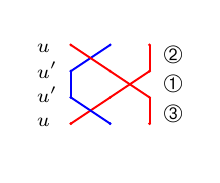
\begin{tikzpicture}[baseline=(current bounding box)]
            \tie[color=red,bull=1,bulletie=0.01,style=solid]{{3,1},{3,0.6667},{2,0.3333},{1,0}}
            \tie[color=blue,bull=1,bulletie=0.01,style=solid]{{2,1},{1,0.6667},{1,0.3333},{2,0}}
            \tie[color=red,bull=1,bulletie=0.01,style=solid]{{1,1},{2,0.6667},{3,0.3333},{3,0}}
 \node at (-0.3,0.06) {$\scriptstyle u\phantom{'}$};
 \node at (-0.3,0.37) {$\scriptstyle u'$};
 \node at (-0.3,0.68) {$\scriptstyle u'$};
 \node at (-0.3,1) {$\scriptstyle u\phantom{'}$};
 \node at (1.3,0.87) {\small\ding{193}};
    \node at (1.3,0.5) {\small\ding{192}};
    \node at (1.3,0.13) {\small\ding{194}};
    \node at (0.5,-0.2) {$\phantom{\scriptstyle i}$};
    \end{tikzpicture}
           &=&
    \;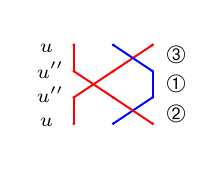
\begin{tikzpicture}[baseline=(current bounding box)]
                \tie[color=red,bull=1,bulletie=0.01,style=solid]{{3,1},{2,0.6667},{1,0.3333},{1,0}}
                \tie[color=blue,bull=1,bulletie=0.01,style=solid]{{2,1},{3,0.6667},{3,0.3333},{2,0}}
                \tie[color=red,bull=1,bulletie=0.01,style=solid]{{1,1},{1,0.6667},{2,0.3333},{3,0}}
     \node at (-0.3,0.06) {$\scriptstyle u\phantom{'}$};
     \node at (-0.3,0.37) {$\scriptstyle u''$};
     \node at (-0.3,0.68) {$\scriptstyle u''$};
     \node at (-0.3,1) {$\scriptstyle u\phantom{'}$};
     \node at (1.3,0.87) {\small\ding{194}};
        \node at (1.3,0.5) {\small\ding{192}};
        \node at (1.3,0.13) {\small\ding{193}};
        \node at (0.5,-0.2) {$\phantom{\scriptstyle i}$};
        \end{tikzpicture}
        &+&
        \;\begin{tikzpicture}[baseline=(current bounding box)]
                    \tie[color=red,bull=1,bulletie=0.01,style=solid]{{1,1},{1,0}}
                    \tie[color=blue,bull=1,bulletie=0.01,style=solid]{{2,1},{2,0}}
                    \tie[color=red,bull=1,bulletie=0.01,style=solid]{{3,1},{3,0}}
           \tie[color=blue]{{2,0.5}}
           \tie[color=red]{{3,0.5}}
           \tie[color=white,bulletie=0.02]{{2,0.5}}
         \node at (-0.3,0.06) {$\scriptstyle u\phantom{'}$};
         \node at (-0.3,1) {$\scriptstyle u\phantom{'}$};
            \node at (1.3,0.5) {\phantom{\small\ding{192}}};
            \node at (0.5,-0.2) {$\phantom{\scriptstyle i}$};
            \end{tikzpicture}       
           \\
D_i^{u,u'}D_{i+1}^{u',u'}D_i^{u',u}&=&\; D_{i+1}^{u,u''}D_{i}^{u'',u''}D_{i+1}^{u'',u} &+&\left(\raisebox{0.4mm}{$\frac{e_{i+2}}{e_{i+1}}$}\right)^{u} \\
\\
    \;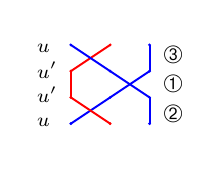
\begin{tikzpicture}[baseline=(current bounding box)]
            \tie[color=blue,bull=1,bulletie=0.01,style=solid]{{3,1},{3,0.6667},{2,0.3333},{1,0}}
            \tie[color=red,bull=1,bulletie=0.01,style=solid]{{2,1},{1,0.6667},{1,0.3333},{2,0}}
            \tie[color=blue,bull=1,bulletie=0.01,style=solid]{{1,1},{2,0.6667},{3,0.3333},{3,0}}
 \node at (-0.3,0.06) {$\scriptstyle u\phantom{'}$};
 \node at (-0.3,0.37) {$\scriptstyle u'$};
 \node at (-0.3,0.68) {$\scriptstyle u'$};
 \node at (-0.3,1) {$\scriptstyle u\phantom{'}$};
 \node at (1.3,0.87) {\small\ding{194}};
    \node at (1.3,0.5) {\small\ding{192}};
    \node at (1.3,0.13) {\small\ding{193}};
    \node at (0.5,-0.2) {$\phantom{\scriptstyle i}$};
    \end{tikzpicture}
           &=&
    \;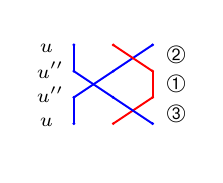
\begin{tikzpicture}[baseline=(current bounding box)]
                \tie[color=blue,bull=1,bulletie=0.01,style=solid]{{3,1},{2,0.6667},{1,0.3333},{1,0}}
                \tie[color=red,bull=1,bulletie=0.01,style=solid]{{2,1},{3,0.6667},{3,0.3333},{2,0}}
                \tie[color=blue,bull=1,bulletie=0.01,style=solid]{{1,1},{1,0.6667},{2,0.3333},{3,0}}
     \node at (-0.3,0.06) {$\scriptstyle u\phantom{'}$};
     \node at (-0.3,0.37) {$\scriptstyle u''$};
     \node at (-0.3,0.68) {$\scriptstyle u''$};
     \node at (-0.3,1) {$\scriptstyle u\phantom{'}$};
     \node at (1.3,0.87) {\small\ding{193}};
        \node at (1.3,0.5) {\small\ding{192}};
        \node at (1.3,0.13) {\small\ding{194}};
        \node at (0.5,-0.2) {$\phantom{\scriptstyle i}$};
        \end{tikzpicture}
        &-&
        \;\begin{tikzpicture}[baseline=(current bounding box)]
                    \tie[color=blue,bull=1,bulletie=0.01,style=solid]{{1,1},{1,0}}
                    \tie[color=red,bull=1,bulletie=0.01,style=solid]{{2,1},{2,0}}
                    \tie[color=blue,bull=1,bulletie=0.01,style=solid]{{3,1},{3,0}}
           \tie[color=red]{{2,0.5}}
           \tie[color=blue]{{1,0.5}}
           \tie[color=white,bulletie=0.02]{{1,0.5}}
         \node at (-0.3,0.06) {$\scriptstyle u\phantom{'}$};
         \node at (-0.3,1) {$\scriptstyle u\phantom{'}$};
            \node at (1.3,0.5) {\phantom{\small\ding{192}}};
            \node at (0.5,-0.2) {$\phantom{\scriptstyle i}$};
            \end{tikzpicture}       
           \\
D_i^{u,u'}D_{i+1}^{u',u'}D_i^{u',u}&=&\; D_{i+1}^{u,u''}D_{i}^{u'',u''}D_{i+1}^{u'',u} &-&\left(\raisebox{0.4mm}{$\frac{e_{i+1}}{e_{i}}$}\right)^{u} \\
\\
\;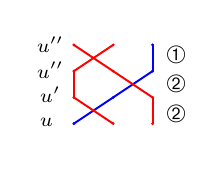
\begin{tikzpicture}[baseline=(current bounding box)]
            \tie[color=blue,bull=1,bulletie=0.01,style=solid]{{3,1},{3,0.6667},{2,0.3333},{1,0}}
            \tie[color=red,bull=1,bulletie=0.01,style=solid]{{2,1},{1,0.6667},{1,0.3333},{2,0}}
            \tie[color=red,bull=1,bulletie=0.01,style=solid]{{1,1},{2,0.6667},{3,0.3333},{3,0}}
 \node at (-0.3,0.06) {$\scriptstyle u\phantom{'}$};
 \node at (-0.3,0.37) {$\scriptstyle u'$};
 \node at (-0.3,0.68) {$\scriptstyle u''$};
 \node at (-0.3,1) {$\scriptstyle u''$};
 \node at (1.3,0.87) {\small\ding{192}};
    \node at (1.3,0.5) {\small\ding{193}};
    \node at (1.3,0.13) {\small\ding{193}};
    \node at (0.5,-0.2) {$\phantom{\scriptstyle i}$};
    \end{tikzpicture}
           &=&
    \;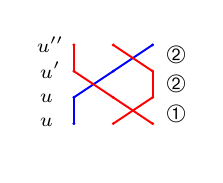
\begin{tikzpicture}[baseline=(current bounding box)]
                \tie[color=blue,bull=1,bulletie=0.01,style=solid]{{3,1},{2,0.6667},{1,0.3333},{1,0}}
                \tie[color=red,bull=1,bulletie=0.01,style=solid]{{2,1},{3,0.6667},{3,0.3333},{2,0}}
                \tie[color=red,bull=1,bulletie=0.01,style=solid]{{1,1},{1,0.6667},{2,0.3333},{3,0}}
     \node at (-0.3,0.06) {$\scriptstyle u\phantom{'}$};
     \node at (-0.3,0.37) {$\scriptstyle u\phantom{'}$};
     \node at (-0.3,0.68) {$\scriptstyle u'$};
     \node at (-0.3,1) {$\scriptstyle u''$};
     \node at (1.3,0.87) {\small\ding{193}};
        \node at (1.3,0.5) {\small\ding{193}};
        \node at (1.3,0.13) {\small\ding{192}};
        \node at (0.5,-0.2) {$\phantom{\scriptstyle i}$};
        \end{tikzpicture}     
           \\
D_i^{u,u'}D_{i+1}^{u',u''}D_i^{u'',u''}&=&\; D_{i+1}^{u,u}D_{i}^{u,u'}D_{i+1}^{u',u''}  \\
\\
\end{array}
\]
\end{table}
\end{document}